\begin{figure*}
  \centering
  \begin{subfigure}[b]{0.42\textwidth}
    \centering
    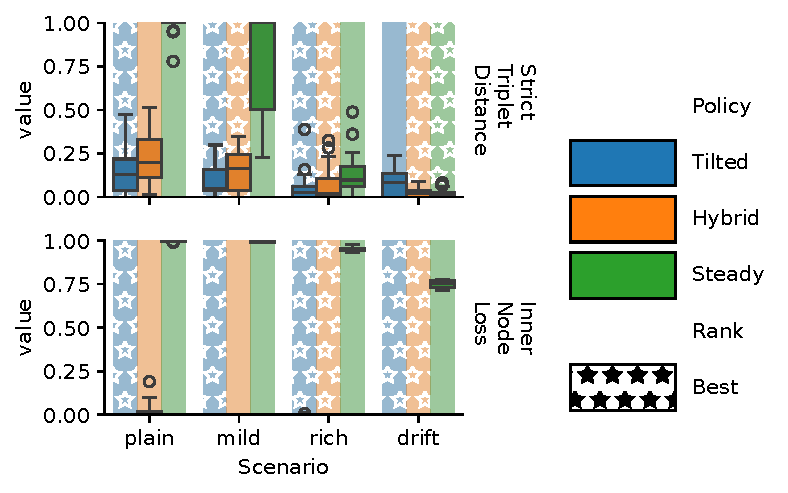
\includegraphics[width=\textwidth]{binder/binder/steady-vs-tilted/teeplots/annotation-size-bits=64+differentia-width-bits=1+downsample=500+hue=policy+num-generations=100000+population-size=65536+post=teed-figure-subplots-adjust-right-0-6-teed-set-titles-row-template-row-name.../+row=variable+score=value+viz=peckplot+x=scenario+x-group=outer+y=value+ext=}
    \caption{TODO}
  \end{subfigure}%
  \begin{subfigure}[b]{0.58\textwidth}
    \centering
    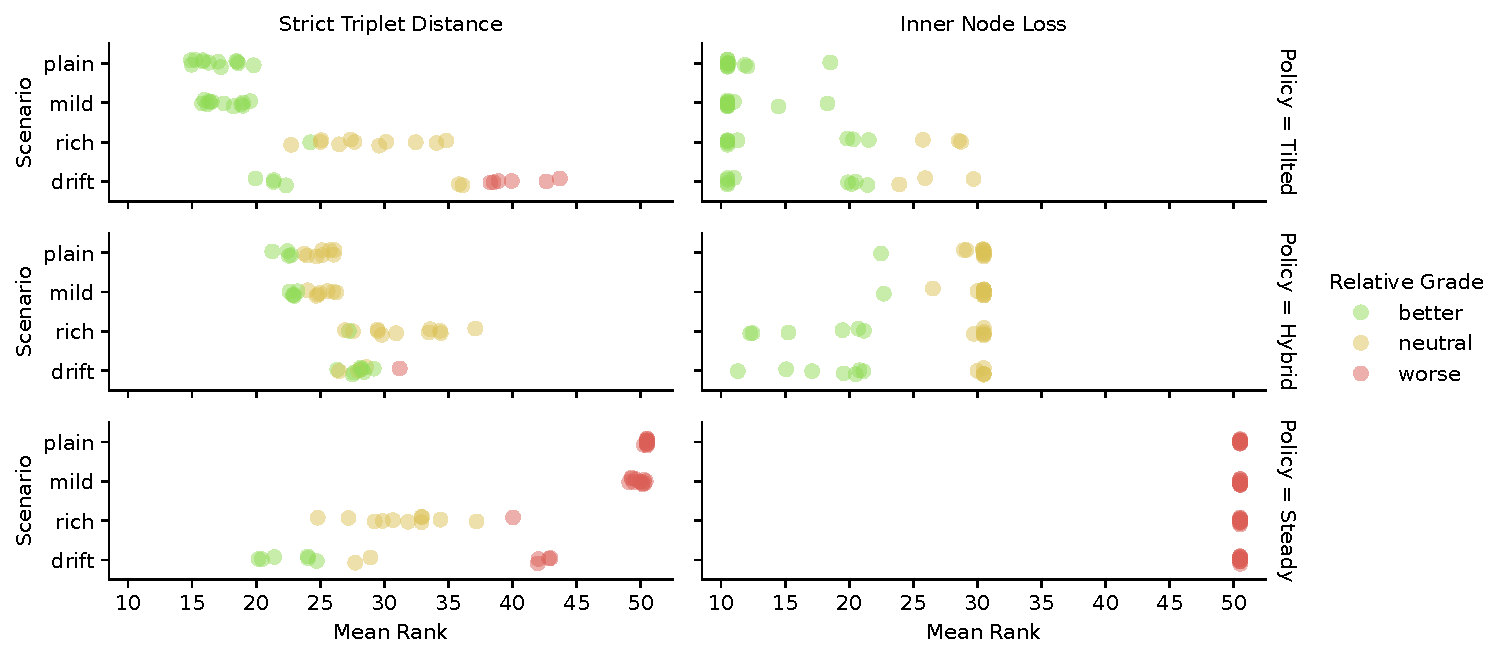
\includegraphics[width=\textwidth]{binder/binder/steady-vs-tilted/teeplots/col=metric+hue=relative-grade+kind=strip+post=teed-set-titles-col-template-col-name+row=policy+viz=catplot+x=mean-rank+y=scenario+ext=}
    \caption{TODO}
  \end{subfigure}
  \caption{%
    \textbf{Steady, tilted, or hybrid?}
  }
  \label{fig:steady-vs-tilted-summary}
\end{figure*}
